\documentclass{article}
% Setup for bibliography
\usepackage[
backend=biber,
style=numeric-comp,
]{biblatex}
\addbibresource{../../references.bib}

% Pretty self explanatory
% We sue this in title bits
\usepackage{datetime}

% Standard math packages / setup
\usepackage{amsmath} 
\usepackage{amsfonts}
\usepackage{amsthm}
\usepackage{amssymb} 
\usepackage{accents}
\usepackage{mathrsfs}
\usepackage{mathtools}

\usepackage{bm}

%\newtheorem{lemma}{Lemma}
%\newtheorem{theorem}{Theorem}
%\newtheorem{definition}{Definition}

% So we can import pngs
\usepackage{graphicx} 

% This gives us nice clickable links 
% https://www.overleaf.com/learn/latex/Hyperlinks#Styles_and_colours
\usepackage{hyperref}
\hypersetup{
    colorlinks=true,
    linkcolor=blue,
    citecolor=blue,
    filecolor=magenta,      
    urlcolor=cyan,
    pdftitle={Monte Carlo Methods (DRAFT)},
    pdfpagemode=FullScreen,
    }
\urlstyle{same}

% Allows us to define colors
% We use this in the next block, listings
\usepackage{color}
\definecolor{dkgreen}{rgb}{0,0.6,0}
\definecolor{gray}{rgb}{0.5,0.5,0.5}
\definecolor{mauve}{rgb}{0.58,0,0.82}

% Allows us to include 
\usepackage{listings}
\lstset{frame=tb,
  language={},
  aboveskip=3mm,
  belowskip=3mm,
  showstringspaces=false,
  columns=flexible,
  basicstyle={\small\ttfamily},
  numbers=none,
  numberstyle=\tiny\color{gray},
  keywordstyle=\color{blue},
  commentstyle=\color{dkgreen},
  stringstyle=\color{mauve},
  breaklines=true,
  breakatwhitespace=true,
  tabsize=4
}

% Adds bulletized outlines with outline environment
\usepackage{outlines}

% Tikz
\usepackage{tikz}

% Colors
\usepackage{xcolor}
\definecolor{uconnblue}{rgb}{0.08, 0.18, 0.28}
\definecolor{intactblue}{rgb}{0.13, 0.26, 0.45}
\definecolor{mastercamred}{rgb}{0.83, 0.01, 0.23}


\usepackage[
  letterpaper,
  left=2cm,
  right=2cm,
  top=2cm,
  bottom=2cm
]{geometry}

\setlength{\parindent}{20pt}

\title{CSE 642: Scribe Notes \\ November 22, 2024}
\author{Russell Bentley}


\begin{document}
\maketitle

\section{Introduction}
Today Linghzi Yang gave an update on his work developing algorithms for the \href{https://cerebras.ai}{Cerbras} chip. Earlier in the semester he presented his work on using a formalized algebra to describe the mapping of problems onto the chip's topology.

\section{Systolic Algorithms for CS2}

This update focused on systolic algorithm design for the CS2 chip. In the literature, a systolic array is a computer architecture composed of tightly coupled processors units, usually in some sort of mesh topology.

The CS2 is a wafer scale accelerator composed of a 2D mesh of independently programmable processing units.
This is compared with a CPU, which has a much smaller number of independent cores that share memory, or a GPU 
which has many cores that execute the same instructions on different data. Another relevant processor type
are TPUs, which have a similar layout but the cores are not independently programmable and are much smaller than Cerebras chips.

Rezaul published paper on tensor core unit architecture, which is relevant \cite{Chowdhury2021}.

The presentation today focused on systolic matrix multiply operations, and how it can be implemented on CS2 using some host device python code and kernels written in a language called csl.

CS2 is network on chip, with $900k$ cores on a chip in a 2D mesh. The actual wafer is around $80$
times bigger than a typical GPU.

There is no shared memory, so data is fed in to cores on the outside, and must be communicated through the network.
With each node also acting as a router in the network, common parallel operations from MPI like broadcast and gather can be implements.

For matrix multiplication, $A \cdot B = C$ we see that data from $A$ flows east and data from $B$ flows south.
At the first time step, $a_{1,1}$ is pushed into $P_{1, 1}$ from the west, and $b_{1, 1}$ is pushed into $P_{1, 1}$ from the north. Computation proceeds like a wave, as data is pushed from one processor to its neighbors.

\begin{center}
  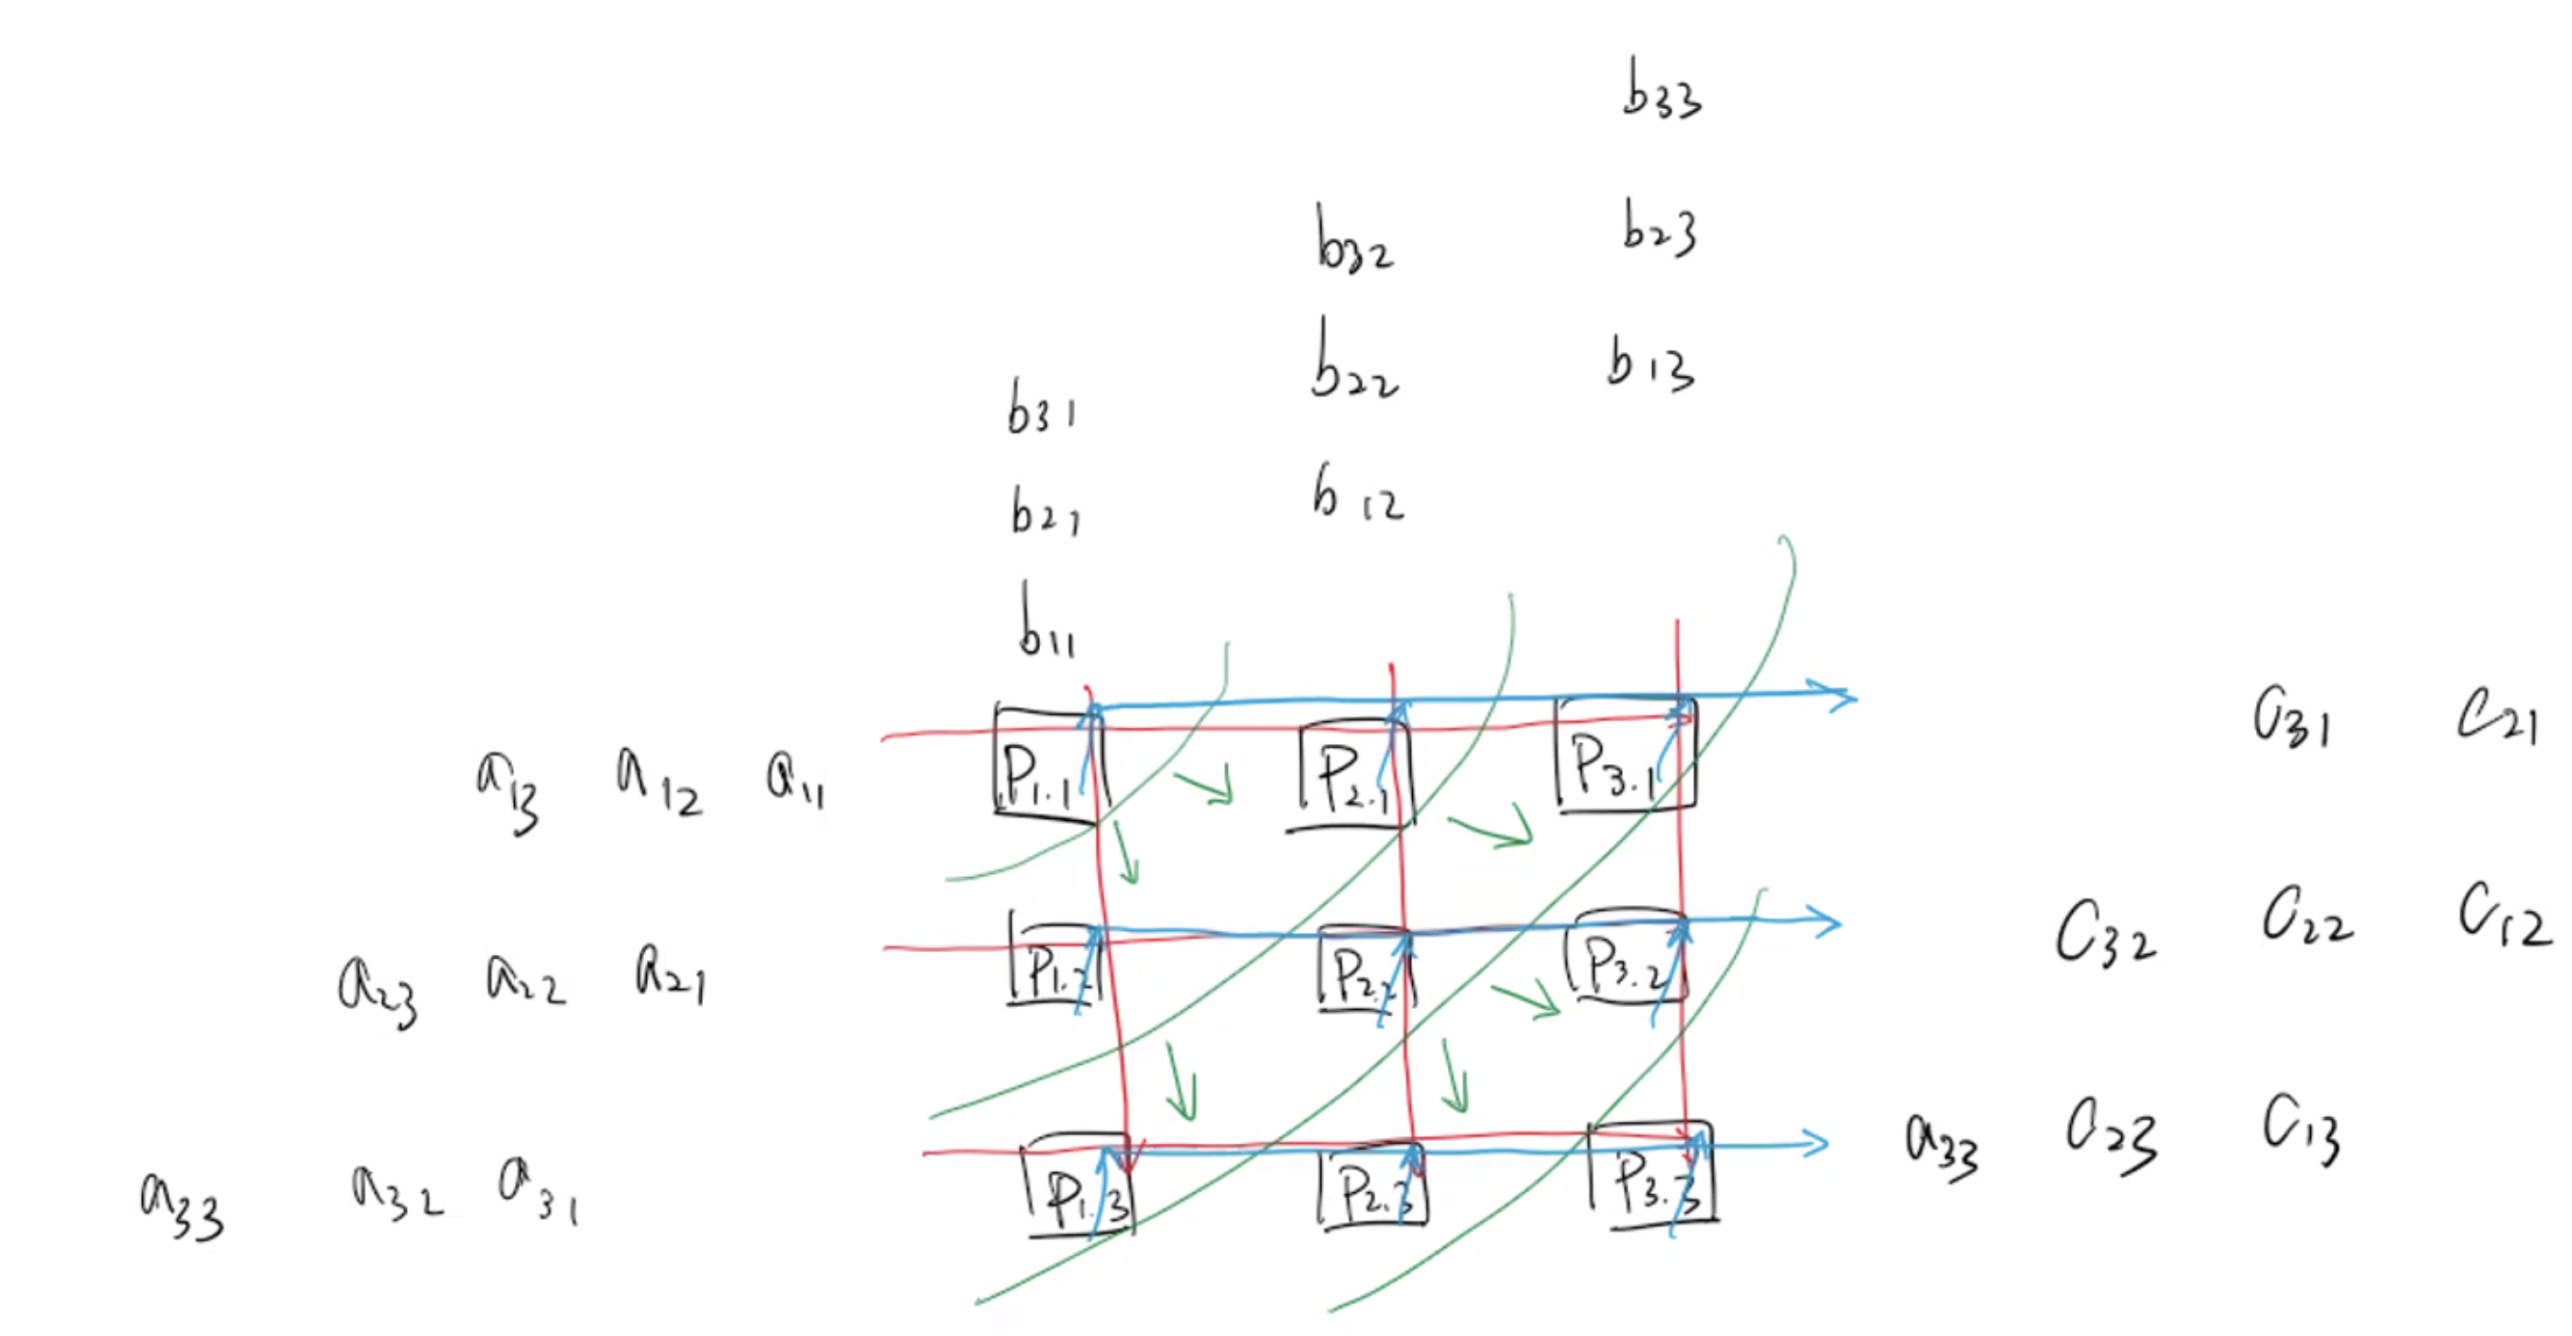
\includegraphics[width=0.5\linewidth]{matrix_multiply.png}
\end{center}

Extra cores are required to communicate data from the host to the grid of kernel cores, as well as data to gather the result and send it back to the host.

\begin{center}
  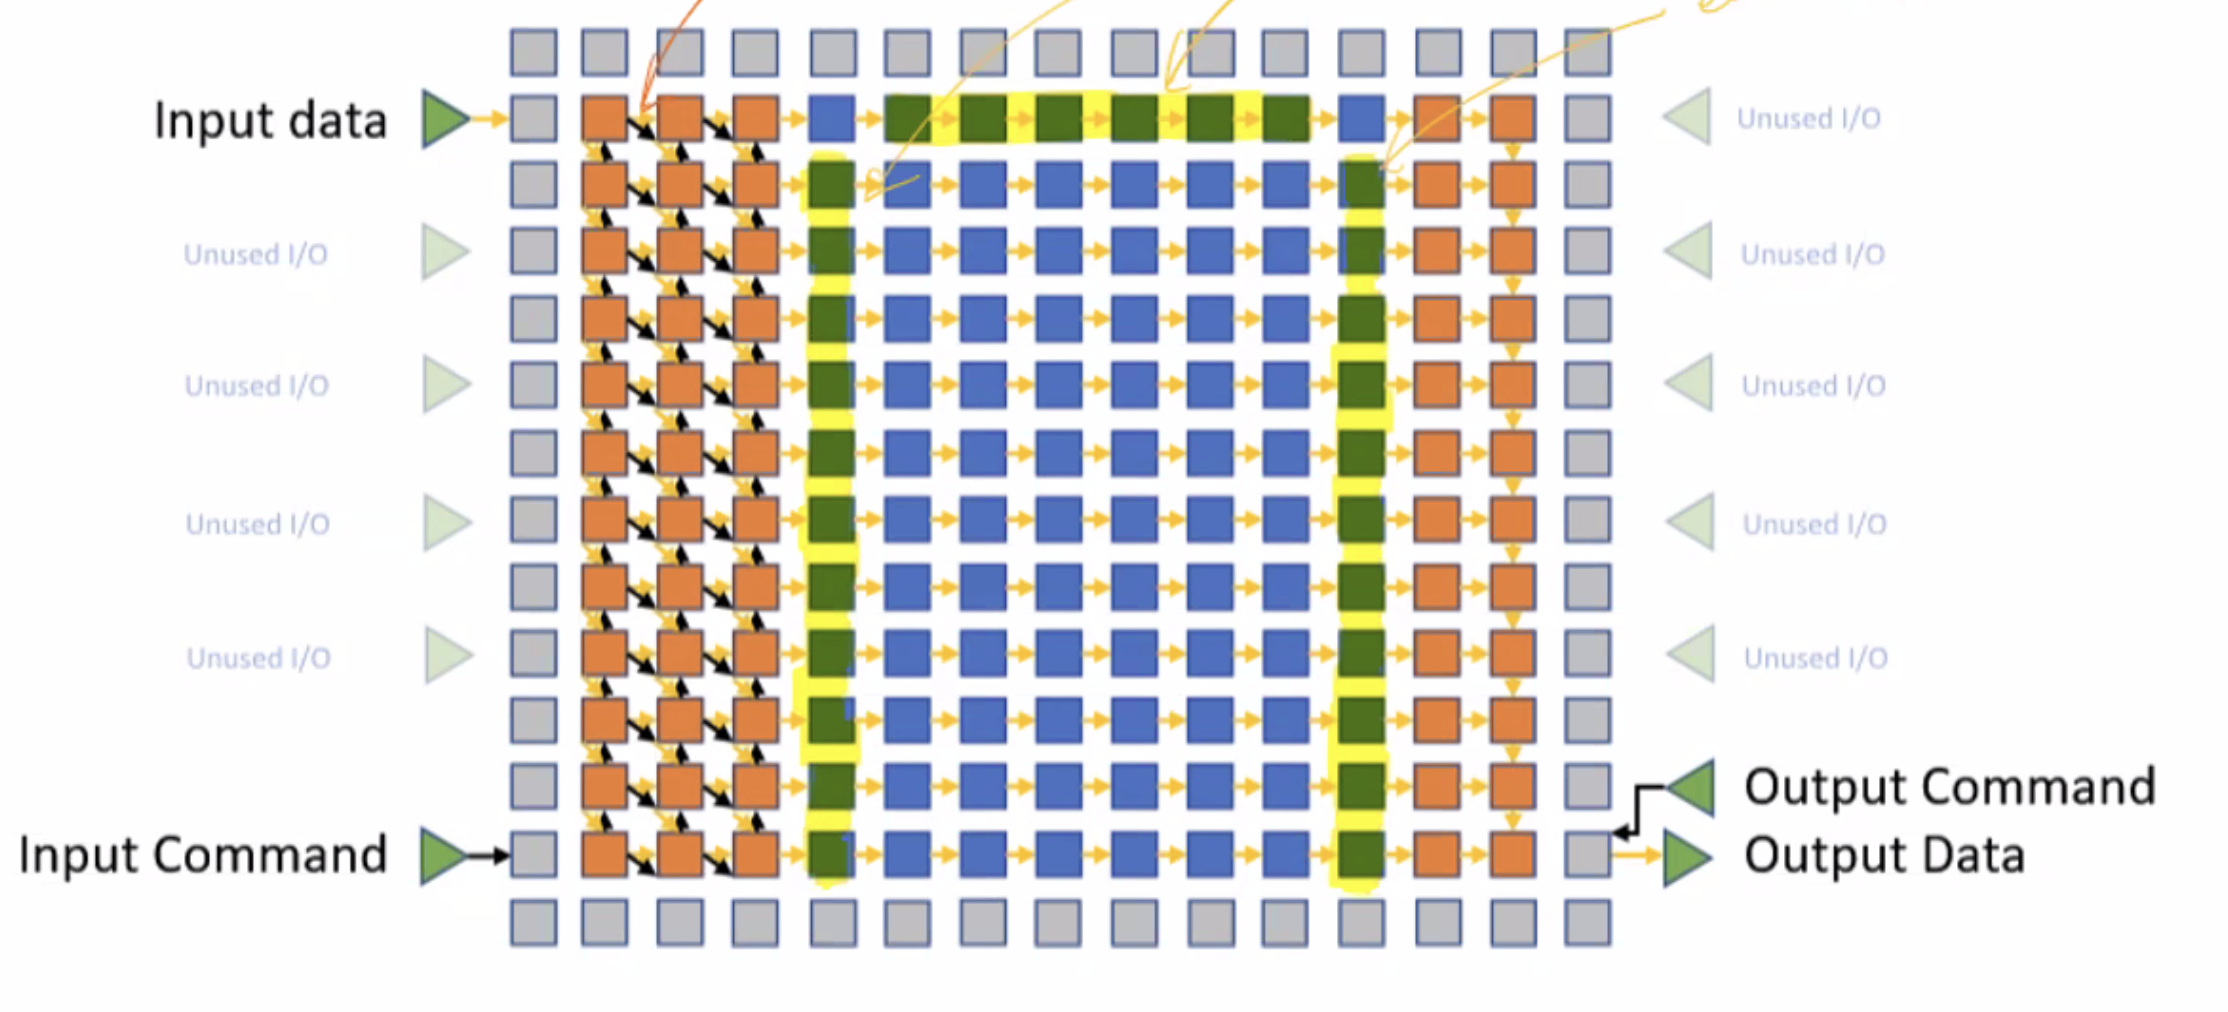
\includegraphics[width=0.5\linewidth]{core_layout.png}
\end{center}

TPU's have a hardcoded array of processing units, like 16 by 16.,
that are not fully not programmable, flow direction is fixed.
Since it’s fixed and small, you need to connect lots of TPUs / GPUs to scale up, 
and it's complicated to network them together.

CS2 has more general processing units (~1ghz) that are fully programmable (with C++ like language). 
Each PE can communicate with all networks, data can flow in any grid direction. 
They can do broadcast / reduce operations like in MPI, 
though this requires each PE implements a router so that data can be propagated to arbitrary PEs.

With TPU networks, only inter node links are programmable. 
With TPU we send individual numbers.
On CS2 we can flow in whole block matrices. 
Each node has enough cache to store 3 80 by 80 matrices.
Typically the grid is broken into region.
A central core region is fully programmable, but we must surround that core with enough nodes to properly feed in data and handle results as they flow out.

Linghzi then walked us through the code required for this matrix multiply operation.
Host side code (written in python), and how it copies data to different cores in the halo.
CSL code starts with a layout that allocated different tasks to different cores.
These tasks / kernels are written in csl as well.
Core tasks are triggered by receiving data.
Each PE has a local scheduler that understands when to execute the task based on data received.
Demonstrated simd fmacs instruction that operates on data in PE cache.

Also demonstrated routing algorithm to flow data, in particular East and south broadcast operations.

Starting to compare results with the Cerebras SDK, which uses a SUMMA based matrix multiply.
Results are early, but currently don't compare favorably with the Cerebras SDK. 
His implementation runs slower and does not exhibit the desired linear scaling.
The issue seems to be feeding data into the chip. 
Currently he only feeds data into two nodes, but could achieve greater throughput by using more input nodes.

\section{Literature Review}
In the 1990s there was alot of systolic algorithm design, old literature can be revived on new hardware.
In general, this time period saw alot of academic exploration for different computer architectures, and much of this work can be translated to the Cerebras architecture.

Back in the 90s these kinds of chips were envisioned but not built yet.
Systolic can only flow data from boundary PEs and globally synchronous.
Data driven becomes wavefront computation, which is what his work is doing.

\begin{center}
  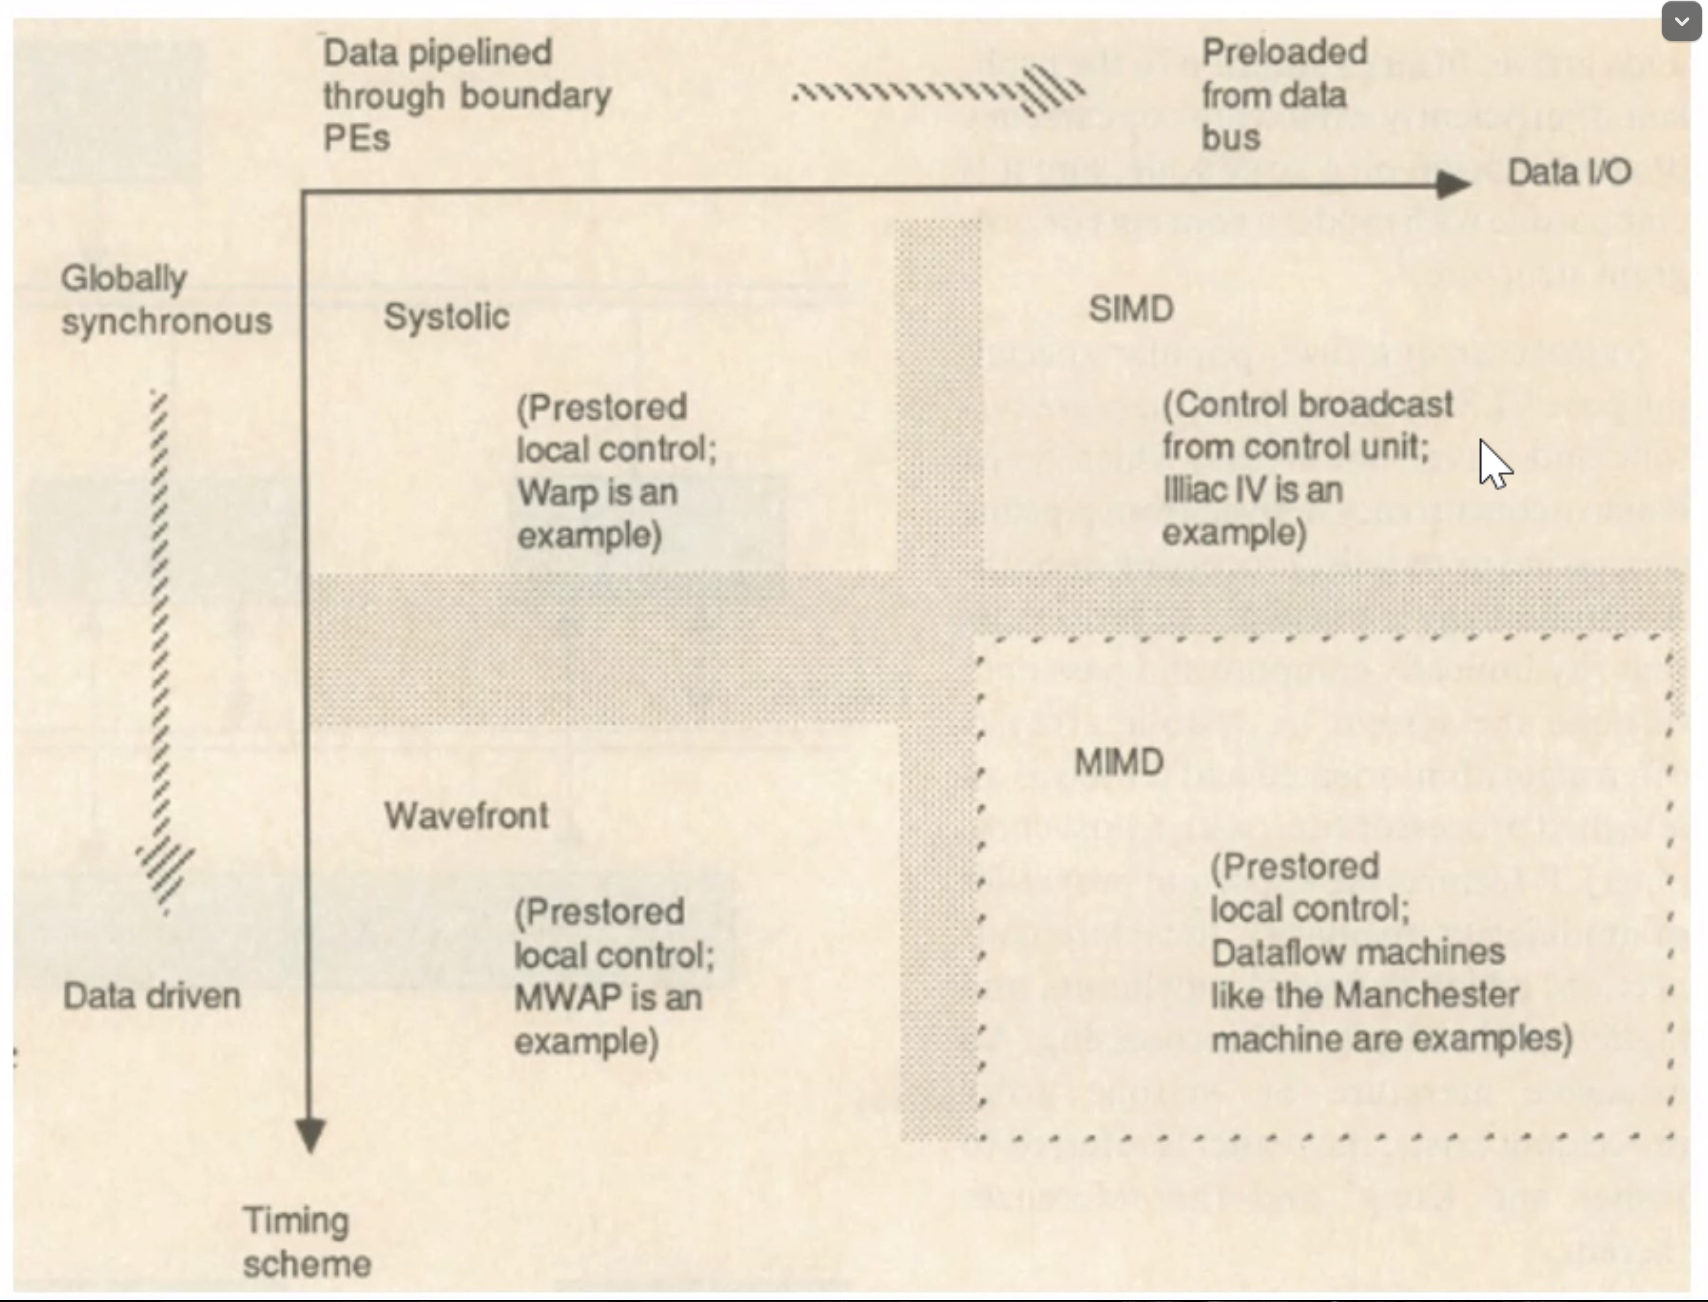
\includegraphics[width=0.5\linewidth]{machine_type.png}
\end{center}

MIMD is dataflow machine, can implement algorithms for the other machine types.
Or General purpose / programmable systolic arrays is another name for this general machine.

So in literature, a variety of algorithms have been explored for these general systolic array machines, 
which can be implemented on MIMD like CS2.
Examples include signal processing, dynamic programming, linear solves, ect.

More generally, dataflow algorithms should be translated to MIMD machines.

Functional programming and stream processing also map well onto CS2.
Functional programming makes sense on MIMD machine, 
each function per PE, data flows between PEs.

\section{Future work and Discussion}

Formal reasoning in systolic algorithm design is an important issue, and was topic of his last talk.
How to formally reason about these algorithms and machines?
Can we use rule based reasoning for verification?
Future work is to use formal reasoning to map systolic algorithms onto the machine, 
and develop a higher level functional language.

Wafer scale hardware could be the future, there was a nice slide with a wafer scale GPU network, where GPUs are directly connected in a grid.
This would allow for embedded super computers that live near the data.

* Strassen layers followed by general matrix multiply for large matrices, could saves like 12\%.
* Can problems over irregular domains be adapted to this architecture, like shortest distance problems.
* What are the big applications you envision? 
    * Speed up LLM / AI is the main focus of Cerebras, currently have fastest LLAMA inference?
    * They have a graph compiler that maps neural networks onto PE grid

\printbibliography

\end{document}


